\chapter{Súčasný stav}

V tejto kapitole popíšeme základné problémy a algoritmy potrebné pri riešení problému korekcie chybových čítaní a metódy implementované v nástrojoch, ktoré sa na tento účel používajú.

\section{Sekvenácia}

DNA sekvencie sú kľúčové dáta v oblasti bioinformatiky. Proces ich získavania je predmetom výskumu už od 70. rokov 20. storočia. V tejto práci budeme opravovať čítania DNA získané sekvenovacím zariadením PacBio RS II. Tieto čítania sa vyznačujú tým, že sú výrazne dlhšie (až do 14 tisíc báz) ako čítania starších sekvenovacích zariadeni (menej ako 1000). Nevýhodou je výrazne vyššia chybovosť, ktora sa pohybuje na úrovni 14\%.

\section{Zarovnávanie čítaní}

Zarovnávanie sekvencií je určenie vzájomnej podobnosti medzy dvoma sekvenciami. Je zložené z dvoch riadkov, pričom riadky zodpovedajú vstup\-ným sekvenciám. V zarovnaní sa do sekvencií vkladajú pomlčky tak, aby malo v stĺpcoch čo najviac rovnakých báz a aby boli riadky rovnakej dĺžky. Príklad zarovnania sa nachádza na obrázku \ref{fig:priklad_zarovnanie}. Na určenie, ktoré zarovnanie je najlepšie, potrebujeme zadefinovať skórovací systém. Skórovací systém priradzuje dvojiciam báz zo zarovnania body podľa toho, či ide o zhodu, substitúciu, deléciu alebo inzerciu. Niektoré algoritmy rozlišujú aj jednotlivé zhody a substitúcie a priradzujú im rôzne hodnoty. Hľadanie zarovnania s najvyšším skóre pre dve sekvencie sa nazýva problém globálneho zarovnania. Problém lokálneho zarovnania sekvencii $A$ a $B$ je hľadanie najlepšieho globálneho zarovania medzi súvislým podreťazcom z $A$ a $B$.

\begin{verbbox}
    CTTCAGT--AGATTG-CC
    -TT-AATCTAGA-TGACC
\end{verbbox}
    
\begin{figure}
    \centering
    \theverbbox
    \caption{Zarovnanie dvoch DNA sekvencií}
    \label{fig:priklad_zarovnanie}
\end{figure}

\subsection{Needleman–Wunsch}

Needlemanov a Wunschov algoritmus slúži na hľadanie najlepšieho globálneho zarovnania medzi dvomi sekvenciami. Využíva sa v ňom princíp dynamického programovania. Na vstupe dostaneme dva reťazce $A$, $B$ nad abecedou \{A, C, T, G\} dlhé $n$, $m$ znakov a výstupom má byť zarovnanie celých reťazcov s najlepším skóre. Pre jednoduchosť zadefinujeme skóre tak, že zhoda má hodnotu $+1$ a substitúcia, inzercia a delécia majú hodnotu $-1$. Potrebujeme dvojrozmerné pole $M$ s rozmermi $n+1$, $m+1$. Na pozícii $[i, j]$ je skóre najlepšieho zarovnania prefixov $A, B$ s dĺžkami $i$ a $j$. 

V tabuľke najprv vyplníme prvý riadok a prvý stlpec. $M[0, 0]$ je 0 (je to zarovnanie dvoch prázdnych reťazcov). Pre ostatné políčka platí, že práve jedna z ich súradníc je nula. Ich najlepšie zarovnanie je toľko substitúcií (resp. delécií), aká je hodnota druhej súradnice. Preto $M[0, i]$ a $M[i, 0]$ má hodnotu $-i$.

Teraz ukážeme, ako vypočítať hodnoty $M[i, j]$ za predpokladu, že poznáme hodnoty políčok s menšími súradnicami. Najlepšie zarovnanie na prefixoch dĺžok $i$, $j$ končí buď dvojicou ($A[i]$, $B[j]$), ($A[i]$, $-$) alebo ($-$, $B[j]$). Ak by končilo dvojicou ($A[i]$, $B[j]$), tak zvyšok zarovnania je zhodný so zarovnaním na prefixoch dĺžok $i - 1$, $j - 1$. Podľa rovnosti $A[i]$ a $B[j]$ je $M[i, j]$ buď $M[i - 1, j - 1]$ + 1 alebo $M[i - 1, j - 1] - 1$. Ak by končilo dvojicou ($A[i]$, $-$), tak zvyšok zarovnania je zhodný so zarovnaním na prefixoch dĺžok $i - 1$, $j$. Hodnota $M[i, j]$ je preto $M[i - 1, j] - 1$. Obdobne vieme vypočítať hodnotu $M[i, j]$ v prípade, že by zarovnanie končilo dvojicou ($-$, $B[j]$). Vieme, že nastane jedna z týchto možností a keďže ide o najlepšie zarovnanie, tak vyberieme najlepšiu z nich. Inak povedané -- hodnota $M[i, j]$ je maximum z hodnôt:

\begin{itemize}
    \item $M[i - 1, j] - 1 $
    \item $M[i, j - 1] - 1 $
    \item $M[i - 1, j - 1] + 1$ ak $A[i] = B[j]$ inak $M[i - 1, j - 1] - 1$
\end{itemize}

\begin{table}
    \centering
    \begin{tabular}{ c || c | c | c | c | c | c | c | c | c | c | c }
            &   & C & T & T & C & A & G & T & A & G & A \\ \hline \hline
            & 0 & 0 & 0 & 0 & 0 & 0 & 0 & 0 & 0 & 0 & 0 \\ \hline 
        T   & 0 &-1 & 1 & 1 &-1 &-1 &-1 & 1 &-1 &-1 &-1 \\ \hline 
        T   & 0 &-1 & 0 & 2 & 1 & 0 &-1 & 0 & 0 &-1 &-2 \\ \hline 
        A   & 0 &-1 &-1 & 1 & 1 & 2 & 1 & 0 & 1 & 0 & 0 \\ \hline 
        A   & 0 &-1 &-2 & 0 & 0 & 2 & 1 & 0 & 1 & 0 & 1 \\ \hline 
        T   & 0 &-1 & 0 &-1 &-1 & 1 & 1 & 2 & 1 & 0 & 0 \\ \hline 
        C   & 0 & 1 & 0 &-1 & 0 & 0 & 0 & 1 & 1 & 0 &-1 \\ \hline 
        T   & 0 &-1 & 2 & 1 & 0 &-1 &-1 & 1 & 0 & 0 &-1 \\ \hline 
        A   & 0 &-1 & 1 & 1 & 0 & 1 & 0 & 0 & 2 & 1 & 1 \\ \hline 
        G   & 0 &-1 & 0 & 0 & 0 & 0 & 2 & 1 & 1 & 3 & 2 \\ \hline 
        A   & 0 &-1 &-1 &-1 &-1 & 1 & 1 & 1 & 2 & 2 & 4 \\
    \end{tabular}
    \caption{Ukážka algoritmu na krátkych sekvenciách}
\end{table}

Pole M teraz môžeme celé vyplniť po riadkoch alebo stĺpcoch. Hodnota $M[n, m]$ je skóre najlepšieho zarovnania sekvencií A a B. Každú hodnotu v poli sme vypočítali v konštantnom čase. Preto časová zložitosť algoritmu je $O(nm)$. Spätným chodom vieme zrekonštruovať zarovnanie s príslušným skóre.

Malou úpravou tohto algoritmu vieme počítať aj lokálne zarovnania. Do poľa by sme namiesto záporných hodnôt ukladali nuly. Najlepšie lokálne zarovnanie v takto vytvorenom poli nájdeme tak, že nájdeme najvačšiu hodnotu v celej matici. Z tohto políčka spätne rekonštrujeme zarovnanie ako v pôvodnom algoritme, ale zastavíme sa na prvej nule. Tento algoritmus sa volá Smithov a Watermanov \citep{smith1981identification}.

\subsection{Jadrá zarovnania}

Zarovnávanie dlhých čítaní v čase $O(nm)$ je časovo aj pamäťovo príliš náročné. Uvedený algoritmus totiž vypĺňa maticu dynamického programovania aj na miestach, ktoré určite vo výslednom zarovnaní nebudú. Jednou zo základných heuristických metód na zrýchlenie procesu zarovnania je hľadanie takzvaných jadier zarovnania. Jadro zarovnania je krátka súvislá zhoda medzi zarovnávanými sekvenciami. Minimálna dĺžka jadier sa nastavuje tak, aby sa ich na sebe prislúchajúich sekvenciách našlo dostatočne veľa a zároven aby bol počet náhodných zhôd bol minimálny. Pri hľadaní jadier zarovnania sa zvyčajne vyrobí vhodná dátová štruktúra z jednej zo sekvencii a následne sa v nej hľadajú súvislé podreťazce ostaných sekvencii. V nasledujúcom texte popíšem najbežnejšie metódy.

\paragraph{Hešovacia tabuľka}

Priamočiare riešenie hľadnia jadier je ukladanie všetkých súvislých podreťazcov dĺžky $k$ v sekvencii spolu s ich pozíciou do hešovacej tabuľky. Kedže rovnaké jadro sa môže nachádzať na viacerých miestach, je potrebné v tabuľke pre jeden reťazec ukladať všetky jeho výskity. Hľadanie jadier prechádzaním všetkých súvislých podpostupností dĺžky $k$ druhej sekvencie a ich náslené vyhľadávanie v hešovacej tabuľke je pomerne rýchly proces. Nevýhodou tejto metódy je pamäťová náročnosť a tiež to, že vieme vyhľadávať len jadrá vopred zvolenej dĺžky.

\paragraph{Sufixové pole}

Sufixové pole je dátová štruktúra použiteľná na vyhľadávanie všetkých výskitov daného podreťazca v reťazci.

Máme reťazec $S$ = $S[0]S[1]S[2]\dots S[n-1]$. Označme $F[i]$ pre $i \in \{0, \dots , n - 1 \}$ sufixy reťazca $S$ začínajúce znakom $S[i]$. Sufixové pole $A$ je pole celých čísel, ktoré na pozícii $j$ obsahuje $i$ také, že existuje $j$ sufixov reťazca lexikografixky menších ako $F[i]$. Binárnym vyhľadávaním sa dajú získať pozície všetkých výskitov hľadaného podreťazca dĺžky $m$ v čase $O(m\lg n)$, avšak využitím pokročilých techník sa dá dosiahnuť časová zložitosť $O(m)$.

Ako príklad uvedieme sufixové pole na reťazci $mississipi$. V tabuľkách \ref{table:suffix_array_suffixes} sú uvedené všetky jeho sufixy usporiadané podľa začiatočnej pozície a lexikograficky. Tabuľka \ref{table:suffix_array_result} zobrazujúca výsledné sufixové pole obsahuje postupne začiatočné pozície lexikograficky usporiadaných sufixov.

\begin{table}
    \begin{subtable}{.5\linewidth}
        \centering
        \begin{tabular}{ l c }
            \toprule
            Sufix   & i \\
            \midrule
            mississippi & 0 \\
            ississippi & 1 \\
            ssissippi & 2 \\
            sissippi & 3 \\
            issippi & 4 \\
            ssippi & 5 \\
            sippi & 6 \\
            ippi & 7 \\
            ppi & 8 \\
            pi & 9 \\
            i & 10 \\
             & 11 \\
            \toprule
        \end{tabular}
        \caption{}
        \label{subtable:suffix_array_suffixes_by_i}
    \end{subtable}
    \begin{subtable}{.5\linewidth}
        \centering
        \begin{tabular}{ l c }
            \toprule
            Sufix   & i \\
            \midrule
             & 11 \\
            i & 10 \\
            ippi & 7 \\
            issippi & 4 \\
            ississippi & 1 \\
            mississippi & 0 \\
            pi & 9 \\
            ppi & 8 \\
            sippi & 6 \\
            sissippi & 3 \\
            ssippi & 5 \\
            ssissippi & 2 \\
            \toprule
        \end{tabular}
        \caption{}
        \label{subtable:suffix_array_suffixes_lexi}
    \end{subtable}
    \caption{Zoznam sufixov zoradený podľa začiatočnej pozície (a) a lexikograficky (b)}
    \label{table:suffix_array_suffixes}
\end{table}

\begin{table}
    \centering
    \begin{tabular}{ l c c c c c c c c c c c c}
        \toprule
        j&0&1&2&3&4&5&6&7&8&9&10&11 \\
        \midrule
        A[j]&11&10&7&4&1&0&9&8&6&3&5&2 \\
        \toprule
    \end{tabular}
    \caption{Sufixové pole na reťazci $mississipi$}
    \label{table:suffix_array_result}
\end{table}

\subsection{DALIGN}

Nástroj DALIGN \citep{myers2014efficient} hľadá lokálne zarovnania medzi dvomi množinami sekvencií. Využíva jadrá zarovnania a heuristiky na nájdenie celého lokálneho zarovnania z jadier.

\paragraph{Rapid Seed Detection}

Máme dve sekvencie $A, B$ dĺžok $N$. Z nich vytvoríme dva zoznamy súvislých $k$-tic spolu s ich pozíciou v rámci sekvencie. Tieto zoznamy lexikograficky usporiadame. Z usporiadaných zoznamov vieme postupným prechádzaním oboch zoznamov naraz vytvoriť zoznam jadier zarovnaní.
Vytváranie zoznamov $k$-tic má lineárnu časovú zložitosť od $N$. Ich následné usporiadanie je v $O(NlogN)$. Hľadanie jadier časovo závisí od ich počtu.

\paragraph{Rapid Local Alignment Discovery}

Po nájdení jadier ich chceme rozšíriť v oboch smeroch po diagonále na čo najväčšie zarovnania. Najprv zadefinujeme pojem editačný graf. Pre dve sekvencie $A$, $B$ dĺžok $M$, $N$ je to graf s vrcholmi ($i$, $j$) z množiny $[0, M] \times [0, N]$. Graf má nasledovné hrany:
\begin{itemize}
\item  ($i-1$, $j$) $\longrightarrow$  ($i$, $j$) pre $i > 0$ s dĺžkou 1 (delécia)
\item  ($i$, $j - 1$) $\longrightarrow$  ($i$, $j$) pre $j > 0$ s dĺžkou 1 (inzercia)
\item  ($i - 1$, $j - 1$) $\longrightarrow$  ($i$, $j$) pre $i, j > 0$ s dĺžkou 0 ak $A[i] = B[j]$, inak 1 (zhoda/substitúcia)
\end{itemize}
Dá sa nahliadnuť, že cesta v grafe jednosnačne definuje jedno zarovnanie a pre každé zarovnanie na sekvenciách $A, B$ existuje  cesta v ich editačnom grafe. Zarovnávací algoritmus na tomto grafe postupne hľada množiny najďalej siahajúcich bodov postupne pre vzdialenosti 1, 2, \dots začinajúc v danom jadre zarovnania. So stúpajúcou vzdialenosťou počet týchto bodov lineárne narastá. Niektorý z nich patrí zarovnaniu ku ktorému výpočet dospeje, ale pre vačšinu vieme s veľkou pravepodobnosťou povedať, že do zarovnania nepatria. V článku sú uvedené dve stratégie orezávania najďalej siahajúcich bodov, ktoré sú vo výslednom zarovnaní s extrémne nízkou pravdepodobnosťou. 

Prvá sa opiera of fakt, že zarovnanie by malo mať na každom úseku určenej dĺžky aspoň nejakú rozumnú koreláciu. Pre každý najďalej siahajúci bod si preto postupne dopočítavame počet zhôd za posledných $C$ hrán na ceste z jadra do daného bodu. To sa dá efektívne implementovať tak, že si v bitovom vektore ukládáme, ktoré z posledných $C$ hrán cesty boli zhodou (1) a ktoré substitúciu/deléciou/inzerciou (0). Počet zhôd potom prepočítame na základe poslednej hrany na ceste a hodnoty vo vektore na pozícii $C$. Po každom kroku sa bitový vector posunie, na začiatok sa pridá nová hodnota, a oreže, aby mal požadovanú dĺžku $C$.

Druhá stratégia je uchovávať len tie body, ktoré sú v rozsahu $L$ antidiagonál od maximálnej dosiahnutej antidiagonály. Body v blízko optimálneho zarovnania mali na ceste od jadra viac zhôd a preto ležia na výrazne vzdialenejších antidiagonálach ako body mimo od optimálneho zarovnania. Tento fakt spôsobuje, že jedna vlna najďalej siahajúcich bodov má tvar hrotu šípu.

Algoritmus skončí, ak dojde na okraj editačného grafu alebo, ak už žiaden najďalej siahajúci bod nespĺňa podmienku lokálnej kvality zarovnania. Orezá\-vacie stratégie robia tento algoritmus heuristickým a len neformálne uvedieme, že má lineárnu časovú zložitosť závislú od dĺžky výsledného zarovnania.

\section{Korekcia čítaní}

Zvýšený výskit chýb sa pri sekvenovaní zariadením PacBio RS II kompenzuje vysokým pokrytím genómu čítaniami. To nám umožní chyby s vysokou úspešnosťou nájsť a opraviť. Opravené čítania sa potom oveľa lepšie použivajú pri ďalšom spracovaní (napríklad rekonštrukcii genómu). Štandardný prístup k tomuto problému je vytvoriť viacnásobné zarovnanie nad opravovaným čítaním z čítaní, ktoré sa s ním prekrývajú. Následne sa pre jednotlivé pozeráme na jednotlivé stlpce a vyberáme najčastejšie hodnoty. V skutočnosti je to trochu komplikovanejšie, keďže algoritmus sa musí vysporiadať s inzerciami a deléciami na referenčnom čítaní aj na pomocných čítaniach.

\subsection{FalconSense}

Algoritmus popísaný v \citep{berlin2015assembling} slúži na opravovanie čítaní použitím zarovnania a elegantne rieši problém medzier v zarovnaní. 

Vstupom je čítanie $T$, ktoré ideme opravovať a množina pomocných čítaní označených $R_1$ až $R_n$. Výstupom je opravené čitanie $T$.

V prvom kroku skúsi zarovnať každé čítanie $R_i$ na $T$. V tomto zarovnaní nepripúšťame substitúcie, takže sa v ňom vyskitujú len zhody, inzercie a delécie.

V druhom kroku vytvorí zoznam štruktúr $(p, d, b) \in  \mathbb{N} \times \mathbb{N} \times \{A, C, G, T\}$. Pre každú bázu $b$ z $R_i$ zarovnanú na bazu z $T$ na pozícii $j$ pridá do zoznamu štruktúru $(j, 0, b)$. Pre všetky bázy z $T$, na ktoré sa nezarovnala žiadna báza z $R_i$ (tj. v danom stlpci zarovnania je pre čitanie $R_i$ ''$-$''), pridá do zoznamu štruktúru $(j, 0, -)$. Pre všetky inzercie vzhľadom na $T$ pridá do zoznamu štruktúru $(j, d, b)$, kde $j$ je pozícia poslednej zhody vramci čítania $T$ a $d$ je počet báz medzi danou bázou a poslednou zarovnanou bázou na $R_i$. 

Zoznam lexikograficky usporiada primárne podľa hodnoty $p$ a ďalej podľa hodnôt $d$ a abecedného poradia $b$. Výslednú sekvenciu získa tak, že spočíta výskit rovnakých trojíc a ak je počet nejakej trojice väčší ako polovica počtu pomocných čítaní, pridá sa na koniec generovanej sekvencie.

Príklad korekcie čítania ATATTAGGC použitím pomocných čítaní ATATACGGC, ATCATCCGGC, ATATACCGAG a ATATAGCCGGC sa nachádza na tabuľke \ref{table:falconsense_example}. Výsledná opravená sekvencia je ATATACGGC.


\begin{table}
    \begin{subtable}{.5\linewidth}
        \centering
\begin{tabular}{ r  l }
	\hline
	čítanie 1 & \verb|ATAT-ACGGC| \\
	podklad   & \verb|ATATTA-GGC| \\
	p =       & \verb|0123455678| \\
	d =       & \verb|0000001000| \\
	\hline
	čítanie 2 & \verb|ATCAT--CCGGC| \\
	podklad   & \verb|AT-ATTA--GGC| \\
	p =       & \verb|011234555678| \\
	d =       & \verb|001000012000| \\
	\hline
	čítanie 3 & \verb|ATAT-ACCGAG-| \\
	podklad   & \verb|ATATTA--G-GC| \\
	p =       & \verb|012345556678| \\
	d =       & \verb|000000120100| \\
	\hline
	čítanie 4 & \verb|ATAT-AGCCGGC| \\
	podklad   & \verb|ATATTAG--G-C| \\
	p =       & \verb|012345666778| \\
	d =       & \verb|000000012010| \\
	\hline
\end{tabular}
        \caption{}
        \label{subtable:falconsense_alignments}
    \end{subtable}
    \begin{subtable}{.5\linewidth}
        \centering
        \begin{tabular}{ l c c }
        	\hline
           	Trojice $(p, d, b)$ & Počty & Výsledná báza \\ \hline \hline
           	 \verb|0, 0, A| & 4 &  \verb|A| \\
           	 \verb|1, 0, T| & 4 &  \verb|T| \\
           	 \verb|1, 1, C| & 1 &  \verb|-| \\
           	 \verb|2, 0, A| & 4 &  \verb|A| \\
           	 \verb|3, 0, T| & 4 &  \verb|T| \\
           	 \verb|4, 0, -| & 4 &  \verb|-| \\
           	 \verb|5, 0, A| & 3 &  \verb|A| \\
           	 \verb|5, 0, -| & 1 &  \verb|-| \\
           	 \verb|5, 1, C| & 3 &  \verb|C| \\
           	 \verb|5, 2, C| & 2 &  \verb|-| \\
           	 \verb|6, 0, G| & 4 &  \verb|G| \\
           	 \verb|6, 1, A| & 1 &  \verb|-| \\
           	 \verb|6, 1, C| & 1 &  \verb|-| \\
           	 \verb|6, 2, C| & 1 &  \verb|-| \\
           	 \verb|7, 0, G| & 4 &  \verb|G| \\
           	 \verb|7, 1, G| & 1 &  \verb|-| \\
           	 \verb|8, 0, C| & 4 &  \verb|C| \\
           	 \hline
        \end{tabular}
        \caption{}
        \label{subtable:suffix_array_suffixes_lexi}
    \end{subtable}
    \caption{Zarovnania pomocných čítaní na opravované čítanie (a) a počty rovnakých trojíc $(p, d, b)$ po lexikografickom usporiadaní (b)}
    \label{table:falconsense_example}
\end{table}

Aby algoritmus nebol ovplyvňovaný oblasťami čítaní, ktoré sa zarovnali len s veľmi malou zhodou použije metódu posuvného okna na spočítanie zhôd v jednotlivých oblastiach čítaní $R_i$. Ak počet zhôd v nejakej oblasti klesne pod vopred určenú hranicu, táto oblasť sa nepoužije pri opravovaní sekvencie. Podobne v oblastiach na $T$, na ktoré sa dobre zarovnalo málo pomocných čítaní $R_i$, sa čítanie rozdelí. Výstupom je potom najdlhšia súvislá (nerozdelená) oblasť.

\subsection{LoRDEC}

Algoritmus LoRDEC vykonáva takzvanú hybridnú korekciu. Pri opravovaní dlhých chybových čítaní má k dispozícii krátke čítania s výrazne nižšou chybovosťou získané z rovnakého živočíšneho druhu. Pred tým ako popíšem tento algoritmus, je vhodné zadefinovať pojem De Bruijnov graf a popísať jeho význam v bioinformatike. 

\paragraph{De Bruijnov graf}

De Bruijnov graf stupňa $k$ je orientovaný graf, ktorého vrcholy reprezentujú všetky súvislé $k$ bázové podpostupnosti sekvencií, z ktorých bol postavený. Hrana z vrcholu reprezentujúceho $k$-ticu $u = s_{1}s_{2}\dots s_{k}$ do vrcholu reprezentujúceho $k$-ticu $v = s_{2}s_{3}\dots s_{k + 1}$ existuje práve vtedy, keď sa v niektorej sekvencii vyskituje $w = s_{1}s_{2}s_{3}\dots s_{k + 1}$. Pre jednotlivé hrany sa zvykne počítať výskit takýchto sekvencii $w$. Na obrázku \ref{fig:debruijngraph} sa nachádza ukážkový de Bruijnov graf stupňa 3 pre sekvencie ACGATG, ACGCATG, TCGATG, TCGCTG a CGCTT. 

\begin{figure}
    \centering
    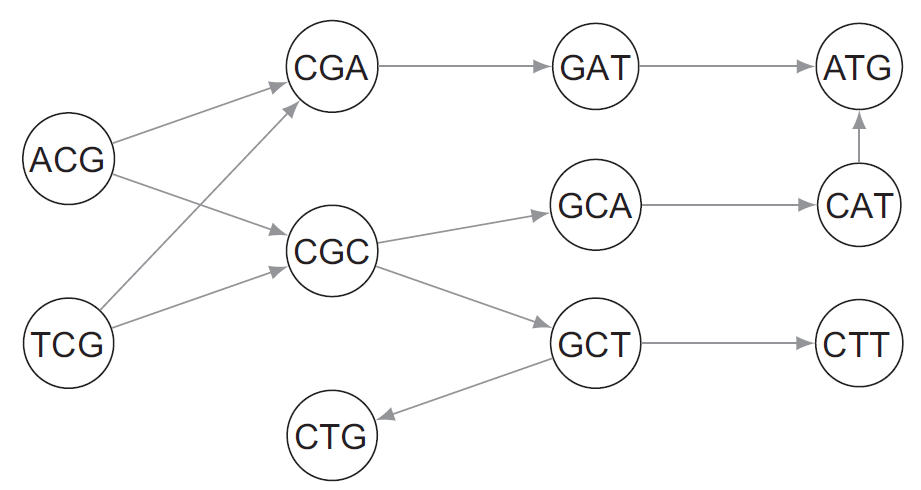
\includegraphics[width=0.6\textwidth]{images/debruijn.png}
    \caption{Ukážka de Bruijnovho grafu}
    \label{fig:debruijngraph}
\end{figure}

De Bruijnove grafy sa používajú pri heuristickom riešení problému zostavovania genómu z čítaní. V prípade, že tieto čítania pochádzajú z jedného vlákna DNA, môžeme problém zostavovania genómu preformulovať na hľadanie Eulerovského ťahu. V prípade, že graf eulerovský ťah neobsahuje, použivajú sa nasledujúce úpravy:
\begin{itemize}
\item Odstraňovanie krátkych slepých ciest, ak im zodpovedajúce sekvencie sú slabo zastúpené vo vstupných čítaniach
\item Znásobňovanie hrán, s výrazne vyšším výskitom v čítaniach
\item Spájanie podciest do jedného vrcholu
\end{itemize}

Vráťme sa späť k nástroju LoRDEC. Ten najprv zostrojí de Bruijnov grav z krátkych čítaní a následne ho použije na opravovanie dlhých chybových čítaní. V prvom kroku sa algoritmus pozrie na všetky $k$-tice vo vstupnom dlhom čítaní. Niektoré z nich sa nachádzajú v de Bruijnovom grafe (označíme ich silné) a niektoré nie (označíme ich slabé). V algoritme sa silné $k$-tice považujú za správne a o slabých sa predpokladá že obsahujú aspoň jednu chybu. V praxi sa ukázalo, že len krátke chybove čítania neobsahujú ani jednu silnú $k$-ticu. Čítania, ktoré neobsahujú ani jednu silnú $k$-ticu program neopravuje.

Predpokladajme teda, že vstupné dlhé čítanie obsahuje aspoň jednu silnú $k$-ticu. Silné $k$-tice rozdeľujú čitanie na súvislé slabé regióny. Algoritmus rôzne pristupuje k vnútorným regiónom (začínajú aj končia silnými regiónmi) a vonkajším regiónom (jeden z koncov je koniec čítania).

\paragraph{Korekcia vnútorných regiónov}

Algoritmus má k dispozícii slabý región ohraničený z oboch strán niekoľkými po sebe idúcimi silnými $k$-ticami a vetviaci limit. Silné $k$-tice slúžia ako začiatočné a koncové vrcholy v de Bruijnovom grafe, čo zaručí, sekvencia zodpovedajúca každej ceste medzi nimi bude zostrojiteľná z krátkych čítaní a zároveň začína a končí správnymi $k$-ticami. Kritérium, podľa ktorého budeme vyberať najlepšiu cestu, je editačná vzdialenosť sekvencie zodpovedajúcej danej ceste od sekvencie slabého regiónu.
Keďže ani silné $k$-tice nemusia byť správne, je vhodné pre každý región vyskúšať viacero dvojíc pre začiatčnú a koncovú $k$-ticu. V tomto algoritme sa pre každú východziu $k$-ticu hľadá najlepšia cesta do $t$ (štandardne nastavené na $t = 5$) najbližších nasledujúcich silných $k$-tic s výnimkou:
\begin{itemize}
\item tých v rovnakej skupine po sebe idúcich silných $k$-tic, lebo tento úsek sa už považuje za správny, korekcia nie je potrebná
\item prekrývajúcich sa; u takýchto $k$-tic hrozí že sú spôsobené opakovaním úseku čítania
\item navzájom príliš vzdialených, lebo by vyžadovali príliš veľa pamete pri hľadaní najlepšej cesty
\end{itemize}

\begin{figure}
    \centering
    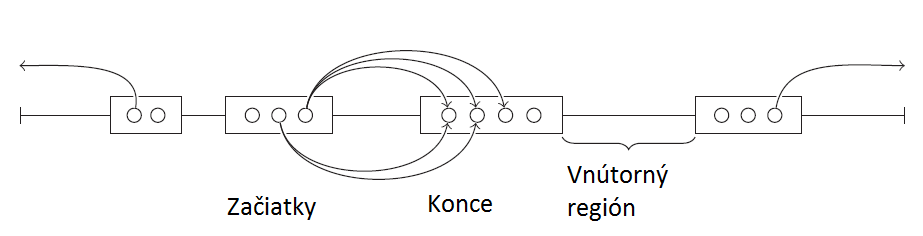
\includegraphics[width=0.8\textwidth]{images/lordec.png}
    \caption{Slabé a silné regióny na chybovom čítaní}
    \label{fig:weakstrongregions}
\end{figure}
Ukážka dvojíc začiatkov a koncov je na obrázku \ref{fig:weakstrongregions}. Uvedený prístup zaručí, že pre každý slabý región sa vyskúša viacero dvojíc pre začiatok a koniec. Na cesty vytvorené nad slabými regiónmi (takzvané mosty) sa pozrieme ako na hrany v novom grafe, ktorého vrcholy sú silné $k$-tice. Samozrejme hrany sú aj medzi susednými prekrývajúcimi sa $k$-ticami. Hrany sú váhované podľa editačnej vzdialenosti medzi sekvenciou regiónu a sekvenciou zodpovedajúcou ceste cez daný slabý región. Použitím Dijkstrovho algoritmu hľadá najkratšiu cestu medzi prvým a posledným slabým regiónom. Hľadanie končí predčasne skončí v prípade, že editačna vzdialenosť najkratšej čiastočnej cesty prekročí určenú hranicu. V prípade, že graf nie je súvislý sa na vhodné miesta pridajú hrany, ktorých váhy sa rovnajú dlžke regiónu medzi $k$-ticami koncových vrcholov. Takto zaručí, že cesta medzi prvou a poslednou silnou $k$-ticou stále existuje.

\paragraph{Korekcia vonkajších regiónov}

Keďže problém prvého a posledného regiónu je symetrický, popíšem len spôsom korekcie toho posledného. Tento región začína jednou silnou $k$-ticou, za ktorou nasleduje región slabých $k$-tic. Na rozdiel od vnútorných regiónov tu nemáme koncovú $k$-ticu, ktorá by jasne ohraničila hľadanú cestu. Prehľadávaním do hĺbky hľadá cestu opravujúcu čo najdlhší prefix koncového regiónu s čo najmenšou editačnou vzdialenosťou. Optimalizácia týchto dvoch parametrov vedie k tomu, že nájdená cesta bude predlžená o úsek s nižšiou koreláciou so zodpovedajúcim úsekom chybového čítania. Tento problém odstránime prezarovnaním najdenej cesty so zodpovedajúcim prefixom a následným skrátením po miesto, kde má zarovnanie najvyššie skóre.











